\chapter{Understanding source code}
\label{chap:understanding}

Aesthetics in source code are thus primarily related to understanding. In the previous chapter, we have highlighted a focus on understanding when it comes to aesthetic standards: whether obfuscating or illuminating, the process of acquiring a mental model of a given computational object is a key determinant in the value judgment as applied to source code. In this chapter, we focus on the reason for which software involves such a cognitive load, before surveying the means—both linguistic and mechanistic—that programmers deploy in order to relieve such a load.

This requirement for understanding, whether in a serious, playful or poetic manner, is related to one of the essential features of software: it must be \emph{functional}. As mentioned in our discussion of the differences between source code and software in the introduction, source code is the latent description of what the software will ultimately do. Similarly to sheet music, or to cooking recipes\footnote{Recipes are a recurring example taken to communicate the concept of an algorithm to non-experts \citep{zeller_algorithms_2020}}, they require to be put into action in order for their users (musicians and cooks, respectively) to assess their value. Therefore, buggy or dysfunctional software is always going to be of less value than correct software \citep{hill_what_2016}, regardless of how aesthetically pleasing the source is. Any value judgment regarding the aesthetics of the source code would be subject to whether or not the software functions correctly, and such judgment is rendered moot if that software does not work.

The assessment of whether a piece of software functions correctly can be broken down in several sub-parts: knowing what the software effectively does, what it is supposed to do, being able to tell whether these two things are aligned, and understanding how it does it. After deciding on a benchmark to assess the functionality of the source code at hand (understanding what it should be doing), one must then determine the actual behavior of the source code at hand once it is executed (understanding what it is actually doing). Due to its writerly nature, one must also understand how a program text does it, in order to modify it.

This chapter examines what goes into understanding source code: given a certain nature of knowledge acquisition, we look at some of the features of computers that make them hard to grasp, and the kind of techniques are deployed in order to address these hurdles. This will have us investigate the relationship of knowing and doing, the nature of computation (what is software?) and its relationship to the world as it appears to us (how does modelling and abstraction translate a problem domain into software?), and the cognitive scaffoldings set up in response to facilitate that task. Ultimately, we show that, given our definition of understanding, the complex nature of software objects and the diverse techniques programmers use to grasp these objects, aesthetics of source code also hold a significant place in this understanding process, a position we develop in \ref{chap:programming}.

The first part will lay out our definition of understanding, presenting it as a dual phenomenon, between formalism and contextualism. Starting with 20\^{th} century epistemology, we will see that theoretical computer science research has favored a dominantly rational, cognitivist perspective on the nature of understanding, eschewing another mode of understanding suggested by craft practices.

Having highlighted this tension, we then turn to how understanding the phenomenon of computation specifically, starting from an ontological level. The ontological approach will show some of the features of software give it the status of an \emph{abstract artifact} \citep{irmak_software_2012}, and thus highlighting in which ways is software a complex object to grasp. We then complement this ontological perspective by a more practical, psychological approach. This will show how such a comprehension takes place for situated programmers, at different skill levels, anticipating how aesthetics can fit in this model.

Finally, we will conclude with the means that programmers deploy to grasp the concepts at play with software: starting from metaphors used by the general public, we will then see to what extent they differ from the metaphors used by programmers in order to understand the systems they build and work with. In the end, particular attention will be paid to their extended cognition the technical apparatuses used in the development and inspection of source code.

\section{Formal and contextual understandings}
\label{sec:formal-contextual-understandings}

This section elaborates our definition of understanding—the process of acquiring a working knowledge of an object\footnote{Or, as Catherine Elgin puts it: "\emph{The cognitive competence involved in understanding is generally characterized as grasping. Propositional understanding involves grasping a fact; objectual understanding consists of grasping a range of phenomena. This seems right. But it is not clear what grasping is. I suggest that to grasp a proposition or an account is at least in part to know how to wield it to further ones epistemic ends}" \citep{elgin_true_2017}}. Such definition relies on two main aspects: a formal, abstract understanding, and a more subjective, empirical one. We will see how the former had some traction in computer sciences circles, while the second gained traction in programming circles. To support those two approaches, we first trace back the genealogy of understanding in theoretical computer science, before outlining how concrete complementary approaches centered around experience and situatedness outline an alternative tradition.

\subsection{Between formal and informal}
\label{subsec:formal-informal}

Understanding can be differentiated between the object of understanding and the means of understanding \citep{elgin_true_2017}. Here, we concern ourselves with the means of understanding, particularly as they are related to the development of computer science. As the science of information processing, the field is closely involved in the representation of knowledge, a representation that programmers then have to make their own.

\subsubsection{Theoretical foundations of formal understanding}
\label{subsubsec:theoretical-understanding}

The theoretical roots of modern computation can be traced back to the early 20\^{th} century in Cambridge were being laid by both philosophers of logic and mathematicians, such as Bertand Russell, Ludwig Wittgenstein, and Alan Turing, as they worked on the formalization of thinking. In their work, we will see that the formalization of knowledge operations are rooted in an operation representation of knowledge.

Wittgenstein, in particular, bases his argumentation in his \emph{Tractatus Logico-philosophicus} on the fact that much of the problems in philosophy are rather problems of understanding between philosophers—if one were to express oneself clearly, and to articulate one's through clear, unambiguous language, a common conclusion could be reached without much effort\footnote{"\emph{    Most questions and propositions of the philosophers result from the fact that we do not understand the logic of our language}" \citep{wittgenstein_tractatus_2010}.}. The stakes presented are thus those of understanding what language really is, and how to use it effectively to, in turn, make oneself understood.

The demonstration that Wittgenstein undertakes is that language and logic are closely connected. Articulated in separate points and sub-points, his work conjugates aphorisms with logical propositions depending on one another, developing from broader statements into more specific precisions, going down levels of abstraction through increasing bulleted lists. Through the stylistic organization of his work, Wittgenstein hints at the possibility to consider language, itself pre-requisite for understanding, as a form of logic This complements the older approach to consider logic as a form of language. In this sense, he stands in the lineage of Gottfried Leibniz's \emph{Ars Combinatoria}, since Leibniz considers that one can formalize a certain language (not necessarily natural languages such as German or Latin), in order to design a perfectly explicity linguistic system. A universal, and universally-understandable language, called a \emph{characteristica universalis} could resolve any misunderstanding issues. Quoted by Russell, Leibniz notes that:

\begin{quote}
    If we had it [a characteristica universalis], we should be able to reason in metaphysics and morals in much the same way as in geometry and analysis\dots{} If controversies were to arise, there would be no more need of disputation between two philosophers than between two accountants [\dots] Let us calculate. \citep{russell_logical_1950}
\end{quote}

Centuries after Leibniz's declaration, Wittgenstein presents a coherent, articulated theory of meaning through the use of mathematical philosophy, and logic. His work also fits with that of Bertrand Russell and Alfred Whitehead who, in his \emph{Principia Mathematica}, attempt to lay out a precise and convenient notation in order to express mathematical notations; similarly, Gottlieb Frege's work attempted to constitute a language in which all scientific statements could be evaluated, by paying particular attention to clarifying the semantic uncertainties between a specific sentence and how it refers to a concept \citep{korte_frege_2010}. Even though these approaches differ from, and sometimes argue with\footnote{See, ironically, Frege's critique of Russell and Whitehead's work, quoted in the Stanford Encyclopedia of Philosophy: "\emph{I do not understand the English language well enough to be able to say definitely that Russell's theory (Principia Mathematica I, 54ff) agrees with my theory of functions of the first, second, etc. levels. It does seem so. But I do not understand all of it. It is not quite clear to me what Russell intends with his designation ___. I never know for sure whether he is speaking of a sign or of its content.}" \citep{linsky_principia_2022}}, one another, we consider them to be part of a broad endeavour to find a linguistic basis to express formal propositions through which one could establish truth-values.

% ϕ!^x

Such works on formal languages as a means of knowledge processing a direct influence in the work on mathematician Alan Turing—who studied at Cambridge and followed some of Wittgenstein's lectures—, as he developed his own formal system for solving complex, abstract mathematical problems, manifested as a symbolic machine \citep{turing_computable_1936}. Meaning formally expressed was to be mechanically processed.

The design of this symbol-processing machine, subsequently known as the Turing machine, is a further step in engaging with the question of knowledge processing in the mathematical sense, as well as in the practical sense—a formal proof to the \emph{Entscheidungsproblem} solved mechanically. Indeed, it is a response to the questions of translation (of a problem) and of implementation (of a solution), hitherto considered a basis for understanding, since solving a mathematical problem supposed, at the time, to be able to understand it.

This formal approach to instructing machines to operate on logic statements then prompted Turing to investigate the question of intelligence and comprehension in \emph{Computing Machinery and Intelligence}. In it, he translates the hazy term of "thinking" machines into that of "conversing" machines, conversation being a practical human activity which involves listening, understanding and answering (i.e. input, process and output; or attention, comprehension, diction) \citep{turing_computing_2009}. This conversational test, which has become a benchmark for machine intelligence, would naively imply the need for a machine to \emph{understand} what is being said.

Throughout the article, Turing does not yet address the need for a purely formal approach of whether or not a problem can be translated into atomistic symbols, as we can imagine Leibniz would have had it which would be provided as an input to a digital computer. Such a process of translation would rely on a formal approach, similar to that laid out in the \emph{Tractatus Logico-philosophicus}, or on Frege's formal language described in the \emph{Begriffschrift}. Following a cartesian approach, the idea in both authors is to break down a concept, or a proposition, into sub-propositions, in order to recursively establish the truth of each of these sub-propositions, and then re-assembled to deduce the truth-value of the original proposition.

Logical calculus, as the integration of the symbol into relationships of many symbols formally takes place through two stylistic mechanisms, the \emph{symbol} and the \emph{list}. Each of the works by Frege, Russell and Wittgenstein quoted above are structured in terms of lists and sub-lists, representing the stylistic pendant to the epistemological approach of related, atomistic propositions and sub-propositions. A list, far from being an innate way of organizing information in humans, is a particular approach to language: extracting elements from their original, situated existence, and reconnecting ways in very rigorous, strictly-defined ways\footnote{Jack Goody develops the influence of notation on cognition: "\emph{[List-making] [\dots] is an example of the kind of decontextualization that writing promotes, and one that gives the mind a special kind of lever on 'reality'.}" \citep{goody_domestication_1977}}.

As inventories, early textbooks, administrative documents as public mnemotechnique, the list is a way of taking symbols, pictorial language elements in order to re-assemble them to reconstitute the world, then re-assemble it from blocks, following an assumption that the world can always be decomposed into smaller, discreete and \emph{conceptually coherent} units (i.e. symbols). One can then decompose a thought in a list, and expect a counterpart to recompose this thought by perusing it. As a symbol system, lists establish clear-cut boundaries, are simple, abstract and discontinuous; incidentally, this makes it very suited to a discreete symbol-processing machine such as the computer \citep{depaz_stylistique_2023}.

With these sophisticated syntactic systems developed a certain approach to cognition, as Turing clearly establishes a possibility for a digital computer to achieve the intellectual capacities of a human brain.

But as Turing focuses on the philosophical and moral arguments to the possibility for machines to think, he does address the issue of formalism in developing machine intelligence. Particularly, he acknowledges the need for intuition in and self-development of the machine in order to reach a level at which it can be said that the machine is intelligent. We now turn to the form of these systems, looking at how their form addresses the problem of clearly understanding and operating on mathematical and logical statements.

Being based on some singular, symbolical entity, the representation of logical calculus into lists and symbols, within a computing environment, becomes the next step in exploring these tools for thinking, in the form of programming languages. Considering understanding through a formal lens can then be confronted to the real world: when programmed using those formal languages, how much can a computer understand?

\subsubsection{Practical attempts at implementing formal understanding}
\label{subsubsec:practical-understanding}

This putting into practice relies on a continued assumption of human cognition as an abstract, logical. Practically, programming languages could logically express operations to be performed by the machine.

The first of these languages is IPL, the Information Processing Language, created by Allen Newell, Cliff Shaw and Herbert A. Simon.  The idea was to make programs understand and solve problems, through "the simulation of cognitive processes" \citep{newell_information_1964}. IPL achieves this with the symbol as its fundamental construct, which at the time was still largely mapped to physical addresses and cells in the computer's memory, and not yet decoupled from hardware.

IPL was originally designed to demonstrate the theorems of Russell's \emph{Principia Mathematica}, along with a couple of early AI programs, such as the \emph{Logic Theorist}, the \emph{General Problem Solver}. As such, it proves to be a link between the ideas exposed in the writing of the mathematical logicians and the actual design and construction of electrical machines activating these ideas. More a proof of concept than a versatile language, IPL was then quickly replaced by LISP as the linguistic means to express intelligence in digital computers (see \ref{subsubsec:computation-end}).

This structure of Lisp is quite similar to the approach suggested by Noam Chomsky in his \emph{Syntactic Structures}, where he posits the tree structure of language, as a decomposition of sentences until the smallest conceptually coherent parts (e.g. Phrase -> Noun-Phrase + Verb-Phrase -> Article + Substantive + Verb-Phrase). The style is similar, insofar as it proposes a general ruleset (or the at least the existence of one) in order to construct complex structures through simple parts.

Through its direct manipulation of conceptual units upon which logic operations can be executed, LISP became the language of AI, an intelligence conceived first and foremost as logical understanding. The use of LISP as a research tool culminated in the \emph{SHRDLU} program, a natural language understanding program built in 1968-1970 by Terry Winograd which aimed at tackling the issue of situatedness—AI can understand things abtractly through logical mathematics, but can it apply these rules within a given context? The program had the particularity of functioning with a "blocks world" a highly simplified version of a physical environment—bringing the primary qualities of abstraction into solid grasp. The computer system was expected to take into account the rest of the world and interact in natural language with a human, about this world (\emph{Where is the red cube?} \emph{Pick up the blue ball}, etc.). While incredibly impressive at the time, \emph{SHDRLU}'s success was nonetheless relative. It could only succeed at giving barely acceptable results within highly symbolic environments, devoid of any noise. In 2004, Terry Winograd writes:

\begin{quote}
    There are fundamental gulfs between the way that SHRDLU and its kin operate, and whatever it is that goes on in our brains. I don't think that current research has made much progress in crossing that gulf, and the relevant science may take decades or more to get to the point where the initial ambitions become realistic.  \citep{nilsson_quest_2009}
\end{quote}

This attempt, since the beginning of the century, to enable thinking, clarify understanding and implement it in machines, had first hit an obstacle. The world, also known as the problem domain, exhibits a certain complexity which did not seem to be easily translated into singular, atomistic symbols.

A critique of formalism as the only way to model understanding was already developed in 1976 by Joseph Weizenbaum. Particularly, he argues that the machine cannot make a judgment, as judgments cannot be reduced to calculation \citep{weizenbaum_computer_1976}. While the illusion of cognition might be easy to achieve, something he did in his development of early conversational agents, of which the most famous is \emph{ELIZA}, the necessary inclusion of morals and emotion of the process of judging intrinsically limit what machines can do\footnote{Joseph Leighton considers judgment has a foundational aspect of understanding, which is the construction of operational knowledge: "\emph{knowledge begins in simple judgments, judgments of feeling or sentience, as yet devoid of explicit conceptual relations, but containing the germs of all higher order functions of thinking.}" \citep{leighton_objects_1907}.}. Formal representation might provide a certain appearance of understanding, but lacks its depth.

Around the same time, however, was developed another approach to formalizing the intricacies of cognition. Warren McCullough's seminal paper, \emph{A logical calculus of the ideas immanent in nervous activity}, co-written with Walter Pitts, offers an alternative to abstract knowledge based on the embodiment of cognition. They present a connection between the systematic, input-output procedures dear to cybernetics with the predicate logic writing style of Russell and others \citep{mcculloch_logical_1990}. This attachment to input and output, to their existence in complex, inter-related ways, rather than self-contained propositions is, interestingly, rooted in his activy as a literary critic\footnote{Even at the Chicago Literary book club, he argues for a more sensuous approach to cognition: \emph{"In the world of physics, if we are to have any knowledge of that world, there must be nervous impulses in our heads which happen only if the worlds excites our eyes, ears, nose or skin."} \citep{mcculloch_delusion_1953}}.

Going further in the processes of the brain, McCullough indeed finds out, in another paper with Letvinn and Pitts \citep{lettvin_what_1959}, that the organs through which the world excites the brain \emph{are themselves} agents of process, activating a series of probabilistic techniques, such as noise reduction and softmax, to provide a signal to the brain which isn't the untouched, unary, \emph{symbolical} version of the signal input by the external stimuli, and nor does it seem to turn it into such.

We see here the development of a theory for a situated, embodied and sensual stance towards cognition, which would ultimately resurface through the rise of machine learning via convoluted neural networks in the 2000s \citep{nilsson_quest_2009}. In it, the senses are as essential as the brain for an understanding—that is, for the acquisition, through translation, of a conceptual model which then enable deliberate and successful action. It seems, then, that there are other ways to know things than to rely on description through formal propositions.

A couple of decades later, Abelson and Sussman still note, in their introductory textbook to computer science, the difficulty to convey meaning mechanically:

\begin{quote}
    Understanding internal definitions well enough to be sure a program means what we intend it to mean requires a more elaborate model of the evaluation process than we have presented in this chapter. \citep{abelson_structure_1979}
\end{quote}

So, while formal notation is able to enable digital computation, it proved to be limited when it came to accurately and expressively  conveying meaning. This limitation, of being able to express formally what we understand intuitively (e.g. \emph{what is a chair?}\footnote{A question addressed by Joseph Kosuth in his conceptual artwork \emph{One and Three Chairs}, 1965}) appeared as computers applications left the domain of logic and arithmetic, and were applied to more more complex problem domains. 

After having seen the possibilities and limitations of making machines understand through the use of formal languages, and the shift offered by taking into account sensory perception as a possible locus of cognitive processes and means of understanding, we now turn to these ways of knowing that exist in humans in a more embodied capacity.

\subsection{Knowing-what and knowing-how}
\label{subsec:knowing-what-how}

With the publication of Wittgenstein's \emph{Philosophical Investigations}, there was a radical posture change from one of the logicians whose work underpinned AI research. In his second work, he disown his previous approach to language as seen in the \emph{Tractatus Logico-philosophicus}, and favors a more contextual, use-centered frame of what language is. Rather than what knowledge is, he looks at how knowledge is acquired and used; while (formal) lanuage was previously defined as the exclusive means to translation concepts in clearly understandable terms, he broadens his perspective in the \emph{Inquiries} by stating that language is \emph{"the totality of language and the activities with which it is intertwined"} and that \emph{"the meaning of a word is its use within language"} \citep{wittgenstein_recherches_2004}, noting context and situatedness as a important factors in the understanding process.

At first, then, it seemed possible to make machines understand through the use of formal languages. The end of the first wave of AI development, a branch of computation specifically focused on cognition, has shown some limits to this approach. Departing from formal languages, we now investigate how an embodied and situated agent can develop a certain sense of understanding.

\subsubsection{Knoweldge and situation}
\label{subsubsec:knowledge-situation}

As hinted at by the studies of McCullough and Levitt, the process of understanding does not rely exclusively on abstract logical processes, but also on the processes involved in grasping a given object, such as, in their case, what is being seen. It is not just what things are, but how they are, and how they are \emph{perceived}, which matters. Different means of inscription and description do tend to have an impact on the ideas communicated and understood.

In his book \emph{Making Sense: Cognition, Computing, Art and Embodiment}, Simon Penny refutes the so-called unversality of formulating cognition as a formal problem, and develops an alternative history of cognition, akin to Michel Foucault's archeology of knowledge. Drawing on the works of authors such as William James, Jakob von Uexküll and Gilbert Ryle, he refutes the Cartesian dualism thesis which acts as the foundation of AI research \citep{penny_making_2019}. A particular example of the fallacy of dualism, is the use of the phrase \emph{implementation details}, which he recurringly finds in the AI literature, such as Herbert Simon's \emph{The Sciences of the Artificial} \citep{simon_sciences_1996}. In programming, to implement an algorithm means to manifest in concrete instructions, such that they are understood by the machine. The phrase thus refers to the gap existing between the statement of an idea, of an algorithm, and a procedure, and its concrete, effective and functional manifestation. This concept of implementation will show how context tends to complicate abstract understanding.

For instance, pseudo-code is a way to sketch out an algorithmic procedure, which might be considered agnostic when it comes to implementation details. At this point, the pseudo-code is halfway between a general idea and the specificity of the particular idiom in which it is inscribed. One can consider the pseudo-code in \ref{code:nielsen_chalktalk}, which describes a procedure to recognize a free-hand drawing and transform it into a known, formalized glyph. Disregarding the implementation details means disregarding any reality of an actual system: the operating system (e.g. UNIX or MSDOS), the input mechanism (e.g. mouse, joystick, touch or stylus), the rendering procedure (e.g. raster or vector), the programming language (e.g. JavaScript or Python), or any details about the human user drawing the circle.

\begin{listing}
    \inputminted{text}{./corpus/pseudocode.txt}
    \caption{Example of pseudo-code attempting to reverse-engineer a software system, ignoring any of the actual implementation details, taken from \citep{nielsen_working_2017}}
    \label{code:nielsen_chalktalk}
\end{listing}

Refuting the idea that pseudo-code, as abstracted representation, is all that is necessary to communicate and act upon a concept, Penny  argues on the contrary that information is relativistic and relational; relative to other pieces of information (intra-relation) and related to contents and forms of presenting this relation (extra-relation). Pseudo-code will only ever make full sense in a particular implementation context, which then affects the product.

He then follows Philip Agre's statement that a theory of cognition based on formal reason works only with objects of cognition whose attributes and relationships can be completely characterized in formal terms; and yet a formalist approach to cognition does not prove that such objects exist or, if they exist, that they can be useful. Uses of formal systems in artificial intelligence in specific, and in cognitive matters in general, is yet another instance of the map and the territory problem—programming languages only go so far in describing a problem domain without reducing such domain in a certain way.

Beyond the syntax of formal logic, there are different ways to transmit cognition in actionable form, depending on the form, the audience and the purpose. In particular, a symbol system does not need to be formal in order to act as a cognitive device. Logical notation exists along with music, painting, poetry and prose. In terms of form, a symbol system of formal logic is only one of many possibilities for systems of forms. In his \emph{Languages of Art}, Nelson Goodman elaborates a theory of symbol systems, which he defines as formal languages composed of syntactic and semantic rules \citep{goodman_languages_1976}, further explored in \ref{sec:aesthetic-cognition}. What follows, argues Goodman, is that all these formal languages involve an act of \emph{reference}. Through different means (exemplification, denotation, resemblance, representation), liguistic systems act as sets of symbols which can denote or exemplify or refer to in more complex and indirect ways, yet always between a sender and a receiver.

Despite the work of Shannon \citep{shannon_mathematical_2001} and its influence on the development of computer systems, communication, as the transfer of meaning from one individual to one or more other individuals, does not exclusively rely on the use of mathematical notation use of formal languages.

From Goodman to Goody, the format of representation also affords differences in what can be thought and imagined. Something that was always implicit in the arts—that representation is a complex and ever-fleeting topic—is shown more recently in Marchand-Zañartu and Lauxerois's work on pictural representations made by philosophers, visual artists and novelists (such as Claude Simon's sketches for the structure of his novel \emph{La Route des Flandres}, shown in \ref{graphic:routedesflandres}) \citep{marchand-zanartu_32_2022}. How specific domains, including  visual arts and construction, engage in the relation between form and cognition is further adressed in chapter \ref{chap:beauty}.

\begin{figure}
    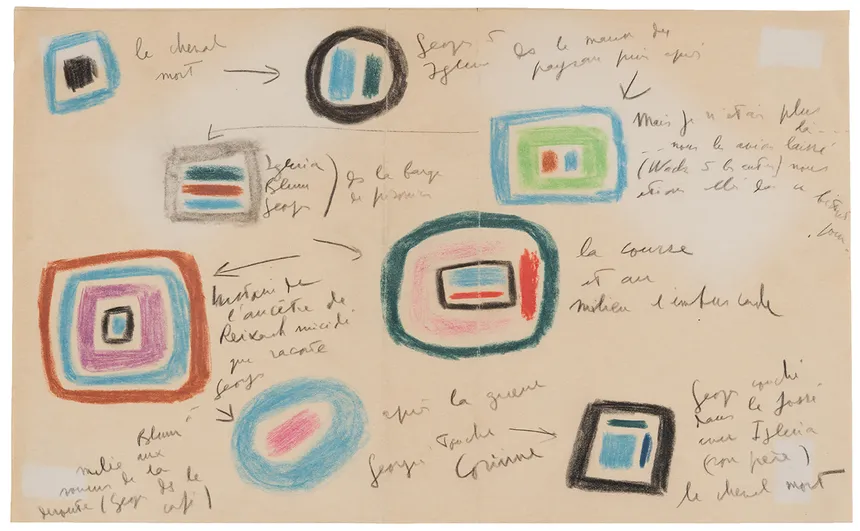
\includegraphics[width=0.8\textwidth,height=\textheight,keepaspectratio,center]{routedesflandres.png}
    \caption{Tentative d'organisation visuelle pour le roman La Route des Flandres, années 1960 - Claude Simon, écrivain}
    \label{graphic:routedesflandres}
\end{figure}

Going beyond formal understanding through logical notation, we have seen that there are other conceptions of knowledge which take into account the physical, social and linguistic context of the agent understanding, as well as of the object being understood. Keeping in mind the recurring concept of craft discussed in \ref{subsubsec:crafting-software}, complete this overview of understanding by paying attention to the role of practice.

\subsubsection{Constructing knowledge}
\label{subsubsec:constructing-knowledge}

There are multiple ways to express an idea: on can use formal notation or draft a rough sketch with different colors. These all highlight different degrees of expression, but one particular way can be considered problematic in its ambition. Formal languages rely on the assumption, that all which can be known can ultimately be expressed in unambiguous terms. First shown by Wittgenstein in the two main eras various eras of his work, we know focus on the ways of knowing which cannot be explicited.

First of all, there is a separation between \emph{knowing-how} and \emph{knowing-that}; the latter, propositional knowledge, does not cover the former, practical knowledge \citep{ryle_concept_1951}. Perhaps one of the most obvious example of this duality is in the failure of Leibniz to construct a calculating machine, as told by Matthew L. Jones in his book \emph{Reckoning with Matter}. In it, he traces the history of philosophers to solve the problem of constructing a calculating machine, a problem which would ultimately be solved by Charles Babbage, with the consequences that we know \citep{jones_reckoning_2016}.

Jones depicts Leibniz in his written correspondence with watchmaker Ollivier, in their fruitless attempt to construct Leibniz's design; the implementations details seem to elude the German philosopher as he refers to the "confused" knowledge of the nonetheless highly-skilled Parisian watchmaker. The (theoretical) plans of Leibniz do not match the (concrete) plans of Ollivier.

These are two complementary approaches to the knowledge of something: to know \emph{what} constructing a calculating machine entails and knowing \emph{how} to construct such a machne. In the fact that Ollivier could not communicate clearly to Leibniz what his technical difficulties, we can see an instance of something which would be theorized centuries later by Michael Polanyi as \emph{tacit knowledge}, knowledge which cannot be entirely made explicit.

Polanyi, as a scientist himself, starts from another assumption: we know more than we can tell. In his eponymous work, he argues against a positivist approach to knowledge, in which empirical and factual deductions are sufficient to achieve satisfying epistemological work. What he proposes, derived from \emph{gestalt} psychology, is to consider some knowledge of an object as the knowledge of an integrated set of particulars, of which we already know some features, by virtue of the object existing in an external approach. This integrated set, in turn, displays more properties than the sum of its parts. While formal notation suggests that the combination of formal symbols does not result in additional knowledge, Polanyi rather argues, against Descartes, that relations and perceptions do result in additional knowledge.

\begin{quote}
    The knowledge of a problem is, therefore, like the knowing of unspecifiables, a knowing of more than you can tell. \citep{polanyi_knowing_1969}
\end{quote}

Rooted in psychology, and therefore in the assumption of the embodimed of the human mind, Polanyi posits that all thought is incarnate, that it lives by the body and by the favour of society, hence giving it a physio-social dimension. This confrontation with the real-world, rather than being a strict hurdle that has to be avoided or overcome, as in the case of SHRDLU above, becomes one of the two poles of cognitive action. Knowledge finds its roots and evaluation in concrete situations, as much as in abstract thinking. In the words of Cecil Wright Mills, writing about his practice as a social scientist research,

\begin{quote}
    Thinking is a continuous struggle between conceptual order and empirical comprehensiveness. \citep{MillsC.WrightCharlesWright2000Tsi}
\end{quote}

Polanyi's presentation of a form of knowledge following the movement of a pendulum, between dismemberment and integration of concepts finds an echo in the sociological work of Mills: a knowledge of some objects in the world happens not exclusively through formal descriptions in logical symbol systems, but involves imagination and phenomenological experience—wondering and seeing. This reliance on vision—starting by recognizing shapes, as Polanyi states—directly implies the notion of aesthetic assessment, such as a judgement of typical or non-typical shapes. He does not, however, immediately elucidate how aesthetics support the formation of mental models at the basis of understanding, only that this morphology is at the basis of higher order of represenations.

Seeing, though, is not passive seeing, simply noticing. It is an active engagement with what is being seen. Mills's quote above also contains this other aspect of Polanyi's investigation of knowledge, and already present in Ollivier's relation with Leibniz: knowing through doing.

This approach has been touched upon from a practical programmer's perspective in section \ref{subsubsec:crafting-software}, through a historical lens but it does also posses theoretical grounding. Specifically, Harry Collins offers a deconstruction of the Polanyi's notion by breaking it down into \emph{relational}, \emph{somatic} and \emph{collective} tacit knowledges \citep{collins_tacit_2010}. While he lays out a strong approach to tacitness of knowledge (i.e. it cannot be communicated at all), his distinction between relational and somatic is useful here\footnote{His definition of collective tacit knowledge touches on the knowledge present in any living species and is impossible to ever be explicited, and is therefore out of scope here.}. It is possible to think about knowledge as a social construct, acquired through social relations: learning the linguo of a particular technical domain, exchanging with peers at conferences, imitating an expert or explaining to a novice. Collective, unspoken agreements and implicit statements of folk wisdom, or implicit demonstrations of expert action are all means of communication through which knowledge gets replicated across subjects.

Concurrently, somatic tacit knowledge tackles the physiological perspective as already pointed out by Polanyi. Rather than knowledge that exists in one's interactions with others, somatic tacit knowledge exists within one's physical perceptions and actions. For instance, one might base one's typing of one's password strictly on one's muscle memory, without thinking about the actual letters being typed, through repetition of the task. Or one might be spotting a cache bug which simply requires a machine reboot, due to experience machine lifecycles, package updates, networking behaviour. Not completely distinct from its relational pendant, somatic knowledge is acquired through experience, repetition and mimeomorphism—replicating actions and behaviours, or the instructions, often under the guidance of someone more experienced.


\spacersmall

We started our discussion of understanding by defining it as the acquisition of the knowledge of a object—be it a concept, a situation, an individual or an artfefact, which is accurate enough that it allows us to predict the behaviour of and to interact with such object.

Theories of how individuals acquire understanding (how they come to know things, and develop operational and conceptual representations of things), have been approached from a formal perspective, and a contexutal one. The rationalist, logical philosophical tradition from which computer science originally stems, starts from the assumption that meaning can be rendered unambiguous through the use of specific notation. Explicit understanding, as the theoretical lineage of computation, then became realized in concrete situations via programming languages.

However, the explicit specification of meaning fell short of handling everyday tasks which humans would consider to be menial. This has led us to consider a different approach to understanding, in which it is acquired through contextual and embodied means. Particularly, we have identified this tacit knowledge as relying on a social component, as well as on a somatic component.

Source code, as a formal system with a high dependence of context, intent and implementation, mobilizes both approaches to understanding. Due to programing's \emph{ad hoc} and bottom-up nature, attemps to formalize it have relied on the assumption that expert programmers have a certain kind of tacit knowledge \citep{soloway1982tapping,soloway_empirical_1984}. The way in which this knowledge, which they are not able to verbalize, has been acquired and is being deployed, has long been an object of study in the field of software psychology.

Before our overview of what the psychology of programmers can contribute on the cognitive processes at play in understanding source code, we must first explicit in which ways software as a whole is a cognitively complex object.

\spacer

\section{Understanding computation}
\label{sec:understanding-computation}

In the previous chapter, we have laid out the groundwork by showing that there are multiple ways to understand something. We now turn to the thing we want to understand. What makes it challenging to understand computation?

First, we will inquire into some distinguishing features of software in terms of levels of abstractions, and in terms of types of complexity. This will highlight some of the theoretical properties that make it hard to understand, such as its relation to hardware, its relation to a specification, and its relation to time and space.

Then, we will shift our perspective to a more abstract point of view, investigating the ontological status of software. This will highlight how software exists as an \emph{abstract artifact}, simultaneously on the ideal, practical and physical plane.

Finally, we will conclude this section by looking specifically at the source code component of software, and how programmers deploy strategies to understand it. Approaching it from a cognitive and psychological perspective, this will give us a better picture of the concrete process of understanding source code—a process which aesthetics are primarily intended to affect.

% the software effect (combination of knowing what (it does) and how (it does it))
\subsection{Software complexity}
\label{subsec:software-complexity}

Software exhibits several particularities, which result in a compex whole—meaning that software possesses several independent components which interact with each other in non-trivial, and non-obvious ways. This subsection focuses on these particularies; that is, on the \emph{properties} of software, and hence how these properties manifest themselves concretely, leading to those complex interactions. We will start by looking at the different levels at which software exists, before turning to the different kinds of complexity which make software hard to grasp.

\subsubsection{Levels of software}
\label{subsubsec:levels-software}

One of the essential aspects of software is that of \emph{implementation}. Implementation is the realization of a plan, the concrete manifestation of an idea, and therefore hints at a first tension in software's multiple facets. It can happen through individuation, instantation, exemplification and reduction \citep{rapaport_philosophy_2005}. On the one side, there is what we will call here \emph{ideal} software, often existing only as a shared mental representation by humans (not limited to programmers), or as printed documentation, as a series of specifications, etc. On the other side, we have \emph{actual} software, which is manifested into lines of code, written in one or more particular languages, and running with more or less bugs.

The relationship between the \emph{ideal} and the \emph{actual} versions of the same software is not straightforward. Ideal software only provides an intent, a guidance towards a goal, assuming, but not guaranteeing, that this goal will be reached. A popular engineering saying is that complements this approach by stating that:

\begin{quote}
    In theory, there is no difference between theory and practice. In practice, there is.\footnote{Sometimes mis-attributed to Richard P. Feynman or Albert Einstein, but traced to Benjamin Brewster, writing in the Yale Literary Magazine of 1882.}
\end{quote}

Actual software, as most programmers know, differs greatly from its ideal version, largely due to the process of implementation, translating the purpose of the software from natural and diagrammatic languages, into programming languages, from what it should do, into what it actually does.

Writing on the myths of computer science, James Moor \citep{moor_three_1978} allows us to think through this distinction between ideal and practical along the lines of the separation between a theory and a model. The difference between a model and a theory is that both can exist independently of one another—one can have a theory for a system without being able to model it, while one can also model a system using \emph{ad hoc} programming techniques, instead of a coherent theory.

Most of the practice of programmers (writing and reading code for the purposes of creating, maintaining and learning software) depends on closing this gap between the ideal and the practical existences of software.

The third level at which software exists is that of hardware. While the ideal version of software is presented in natural language, diagrams or pseudo-code, and while the practical version of software exists as executable source code, software also exists at a very physical level—that of transistors and integrated circuits.

The distinction between software and hardware has been examined thoroughly \citep{kittler_there_1997,chun_sourcery_2008,rapaport_philosophy_2005}, but never strictly defined. Rather, the distinction between what is hardware and what is software is relative to where one draws the line: to a front-end web developer writing JavaScript, the browser, operating system and motherboard might all be considered hardware. For a RISC-V assembly programmer, only the specific CPU chip might be considered hardware, while the operating system being implemented in C, itself compiled through Assembly, would be considered software. A common definition of hardware, as the physical elements making up the computer system, overlooks the fact that software itself is, ultimately, physical changes in the electrical charge of the components of the computer.

Software can be characterized the dynamic evolution of logical processes, described as an ideal specification in natural languages, as a practical realization in programming languages, and in specific states of hardware components. Furthermore, the relations between each of these levels is not straightforward: the ideal and the practical can exist independently of each other, while the practical cannot exist independently of a machine\footnote{Even if that machine is a \emph{virtual machine}, further complicating the boundary between hardware and software}.

\subsubsection{Types of complexity}
\label{subsubsec:types-complexity}

Along with different levels of existence needed to be taken into account by the programmer, software also exhibits specific kinds of complexity. Our definition of complexity will be the one proposed by Warren Weaver. He defines problems of (organized) complexity as those which involve dealing simultaneously with a sizable number of factors which are interrelated into an organic whole \citep{weaver_science_1948}\footnote{As opposed to disorganized complexity, which are dealt with statistical tools.}. Specifically, there are four different types of software complexity that we look at: conceptual complexity, modeling complexity, temporal complexity and spatial complexity.

Conceptual complexity, as refered to by Lando et. al. in their ontology of computer programs, addresses the necessity to model complex objects at different abstraction levels \citep{lando_general_2007}. As mentioned above, software exists at least on three somewhat distinct levels: the ideal, the practical, and the physical. This means that software, in its source code representation, should be able to provide the programmer with tools to engage with its intended function and its actual function at each of these levels. For instance, comments might relate to the ideal behaviour of the software, function declarations to its practical behaviour, while macro definitions can point to the specific hardware on which the code is run.

% insert a table of C code where you see some comment, some function, and some macro

Additionally, conceptual complexity involves the distinction of the different elements of a computer program at the source code level, and keep track of their ontological status, sometimes independently from its level of existence. This distinction should be made notwithstanding the naming conventions assigned by different platforms, vendors, or programming languages, and rather based on ontological properties of the elements at hand. For instance, the distinction between \emph{endurants} and \emph{perdurants} by Lando et. al. focuses on the temporal dimension of software components (i.e. a data structure declaration has a different temporal property than a function call). Here we have a second, complementary frame to that of the levels of existence, through which we can analyze source code; being somewhat related but an exact mapping of one another.

Modeling complexity addresses the hurdles in translating a non-discrete, non-logical object, event, or action, into a discreete, logical software description through source code. Indeed, the history of software development is also the history of the extension of the application of software, and the hurdles to be overcome in the process. From translation of natural languages \citep{poibeau_machine_2017}, to education \citep{watters_teaching_2021} or psychological treatment \citep{weizenbaum_computer_1976}, it seems that problems that seem somehat straightforward from a human perspective become more intricate once the time for implementation has come.

we have seen so far the complexities tied to the conceptualization and modelization of the components of software. Two other significant contributions to the cognitive load of understanding software happen are more closely related to the concrete execution of the software—temporal and spatial complexity.

Temporal complexity relates to the discrepancy between the way the computer was first thought of —i.e. as a Turing machine which operates linearly, on a one-dimensional tape—and further technological developments. Originally, the Turing machine would involve the ability for the head of the machine to jump at different locations. This meant that the execution and reading of a program would be non-linear, jumping from one routine to another across the source code. Such an entanglement is particulary obvious in Ben Fry's Distellamap series of visualizations of source code (\ref{graphic:pacman-visualization} represents the execution of the source code for the arcade game Pac-Man), and led to Edsger W. Dijkstra's statement on the harmfulness of such jumps on the cognitive abilities of programmers.


\begin{figure}
    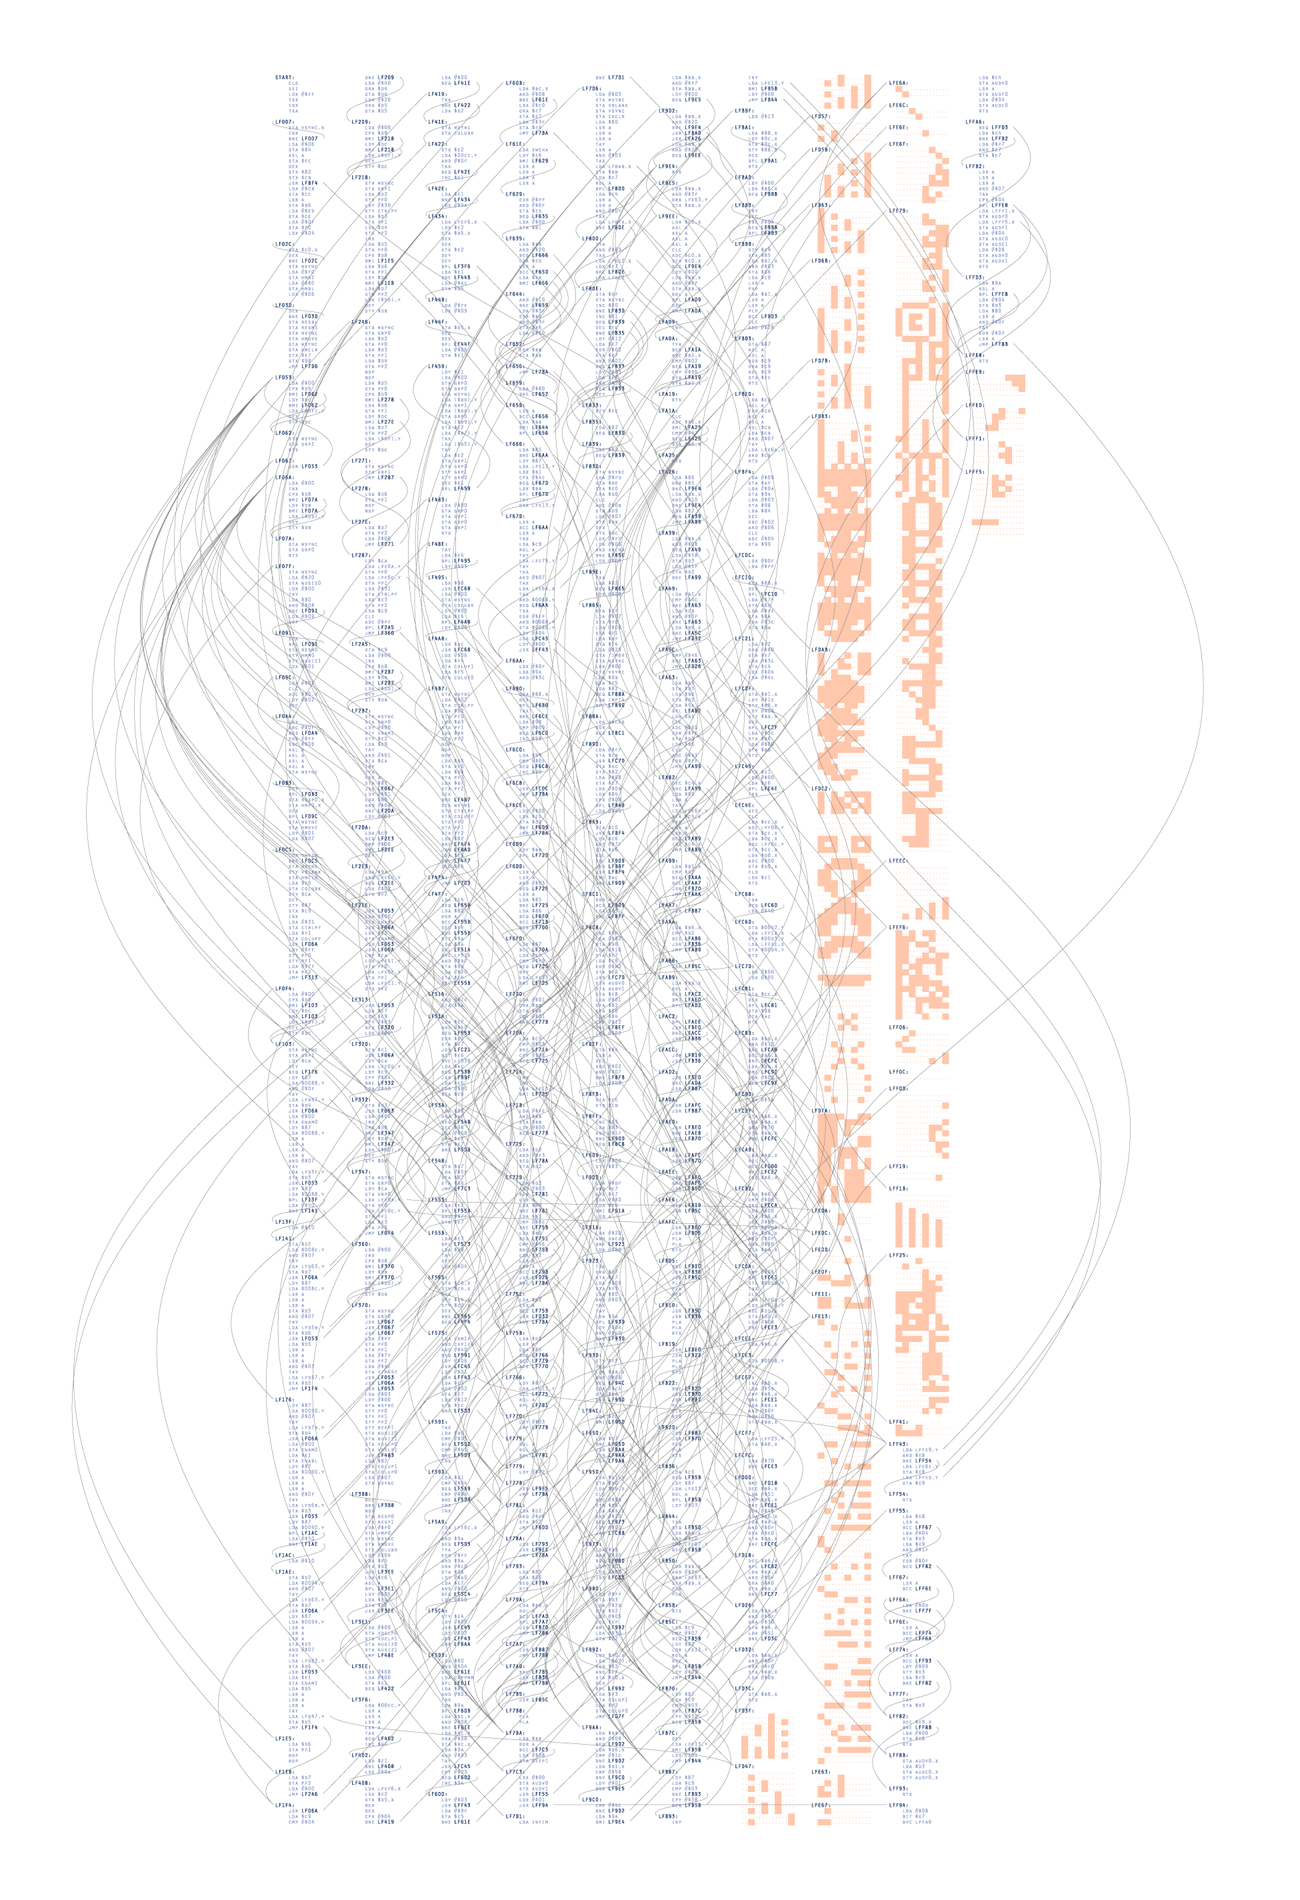
\includegraphics[width=0.8\textwidth,height=\textheight,keepaspectratio,center]{distellamap_pacman.png}
    \caption{Visualization of the execution of Pac-Man's source code}
    \label{graphic:pacman-visualization}
\end{figure}

Later on, the introduction of multi-core architecture for central processing units in the late 2000s has enabled the broad adoption of multithreading and threaded programming. As a result, source code has transformed from a single non-linear execution to a multiple non-linear process, in which several of these non-linear executions are happening in parallel. Keep tracking of what is executing when on which resource is involved in problems such as \emph{race conditions}, when understanding the scheduling of events (each event every e.g. 1/18000000th of a second on a 3.0 Ghz CPU machine) becomes crucial to ensuring the correct behaviour of the software.

Conversely, the locii of the execution of software creates contributes to those issues. Software can be (dis-)located across multiple files on a single machine, on multiple processes on a single machine, or on multiple processes on multiple machines (on a local-area or wide-area network) \citep{berry_philosophy_2011}. This further fragments the interface to the object of understanding. For instance, the asynchronicity of requesting and processing information from distinct processes is a spatial separation of code which has temporal implications (e.g. due to network latency).

\spacer

Software, then, exhibits certain properties which make it difficult to understand, from conception to application: software in the real-world involves implementing concepts that lose in translation, interfacing the world through discreete representations, and following the execution of these representations through space and time, as software executes more and more in a distributed and parallel fashion.

% the philosophical enquiries
\subsection{Software ontology}
\label{subsec:software-ontology}

Now that we have clarified some of what software complexity consists of, we will frame these difficulties in a philosophical context, more specifically the philosophy of technology. We will investigate how these complexities can be seen as stemming from the nature of technology itself, and how this allows us to reconnect it to aesthetic perception. Before moving back to practical inquiries into how specific individuals engage with this nature, this section will help provide a theoretical backdrop, framing technology as a relational practice, complementing other modes of making sense of and taking action on the world. This conceptual framework will start with an investigation into the denomination of software as an \emph{abstract artifact}, followed by an analysis of technology as a specific mode of being, and concluding on how it is related to an aesthetic mode of being.

\subsubsection{Software as abstract artifact}
\label{subsubsec:abstract-artifact}

When he coins the phrase \emph{abstract artifact}, Nurbay Irmak addresses software partly as an abstract object, similar in his sense to Platonic entities\footnote{Like Joseph Kosuth's aforementioned trio of chairs..}. Nonetheless, he also grants that software holds spatio-temporal properties \citep{irmak_software_2012}. Indeed, software does need to exist as an implementation, in the form of source code \citep{suber_what_1988}; this implies that software is composed of files, has a beginning (start) and an end (exit), meanwhile also representing ideas of structure and procedure which go beyond these limitations of being written to a disk and having an execution time. Typically, the physical aspects of software (its manifestation as source code) can be changed\footnote{A process called \emph{refactoring}.} without changing any of the ideas expressed by the software\footnote{A phenomenon one can also observe in natural languages, in which one can radically change a syntax without drastically changing the semantics of a sentence.}.

Complementing Irmak, Colburn's phrasing is that of a \emph{concrete abstraction}, an oxymoron which echoes the tensions denoted by the concept of an abstract artifact.

He grounds these tensions in the distinction between a medium of execution (a—potentially virtual—machine) and a medium of description (source code). He considers that, while any high-level programming language is already the result of layers of abstraction, such language gets reduced to the zeroes and ones input to the central processing unit \citep{colburn_philosophy_2000}. Here, he sees the abstraction provided by languages ultimately bound to the concrete state of being of hardware and binary. And yet, if we follow along along his reasoning, these representations of voltage changes into zeroes and ones are themselves abstractions over yet another concrete, physical event.

Writing on computational artefacts, of which software is a subset, Raymond Turner formalizes this specificity of in a three-way relationship. Namely, abstract artefact A is an implementation in medium M of the definition F. For instance, concerning the medium:

\begin{quote}
    Instead of properties such as \emph{made from carbon fiber}, we have properties such as \emph{constructed from arrays in the Pascal programming language, implemented in Java}. \citep{turner_computational_2018}
\end{quote}

This metaphor provides an accurate but limited account of the place of source code within the definition of software: the Java implementation is itself a definition implemented in a specific bytecode, etc. Nonetheless, source code is that which gives shape to the ideas immanent in software—through a process of concretization—and which hides away the details of the hardware—through abstraction. This metaphor of \emph{abstract artifact} thus helps to clarify the tensions within software, and to locate the specific role of source code within the different moving parts of definition, medium and model.

Recalling that software has a somewhat unique relatoin between its \emph{functional} properties (i.e. purpose that are intended to be achieved through their use) and \emph{structural} ones (physical configuration which are involved in the fullfilment of the functional purpose) \citep{turner_computational_2018}, it remains nonetheless a kind of technology. As such, it also holds some of the specifities of this lineage, into which we can extend our inquiry.

\subsubsection{Software as a relational object}
\label{subsubsec:software-relational}

The technological object underwent a first qualitative shift during the European Industrial Revolution, and a second one with the advent of computing technologies. The status of its exact nature is therefore a recent object of inquiry. Here, we will start from Gilbert Simondon's understanding of technology as a \emph{mode}, in order to ultimately contrast it with the \emph{aesthetic mode}.

According to Simondon, the technical object is a relation between multiple structures and the result of a complex operation of various knowledges \citep{simondon_mode_1958}, some scientific, some practical, some social, some material. The technical object is indeed a scientific object, but also a social object and an artistic object at the same time. Differentiated in its various stages (object, individual, system), it is therefore considered as relational, in that its nature changes through its dependance and influence on its environment.

From this relational standpoint, one could complement Bernard Stiegler's statement that technology is a dynamic of organized, but inorganic matter \citep{stiegler_technics_1998}, if we are to consider inorganized matter to include social influences, personal practices, and forms of tacit and explicit knowledges. That is, the ambiguity of the technical object is that it extends beyond itself as an object, entering into a relation with its surrounding environment, including the human individual which makes use of it. Up until the invention of the clock, technology remained bound to practical matter. With the invention of seconds, its action reached into another domain—that of mechanical operation on abstract ideas \citep{mumford_technics_1934}.

The domain of abstract ideas was hitherto reserved to different modes than technology: that of religion and philosophy, and technology holds a particularly interesting relation with these two. According to Simondon, philosophy followed religion as a means of relating to, and making sense of, the abstract such the divine and the ethical. Tracing back the genesis of the technological object, e writes that the technical mode of existence is therefore just another mode through which the human can relate to the world, similar to the religious, the philosophical, and the aesthetic mode\citep{simondon_mode_1958}.

While both technology, religion and philosophy are based on theoretical knowledge, technology is specifically manifested in practice, and while it is manifested in ethics, in religion. Technology is thus seen as the combination of a theory of knowledge and a theory of action. Such a combination has since been extended into the abstract domain, leading to computers, as a form of technology through which \emph{meaning is mechanically realized}.

%TODO add a section on yuk hui here, for the digital objects.

Simondon complements the technical and the religious modes with the aesthetic mode, and as such counter-balances the apparent split between technics and religion by striving for unity and totality, for the balance between the objective and the subjective. Yet, rather than being a monadic unity of a single principle, Simondon considers the aesthetic mode as a unifying a network of relationships, a form of organizing Stiegler's inorganized matter. He further argues that the aesthetic mode goes beyond taste and subjective preference, into a fundamental aspect of the way in which human beings relate to the world around them. An aesthetic object therefore acquires the property of being beautiful by virtue of its relationships, of its connections between the subject and the objective, between one's history and one's perceptions, and the various elements of the world, and the actions of the individual. Finally, the aesthetic thought when related to the technical object consists in preparing the communication between different communities of users, between different perspectives on the world, and different modes of action upon this world. An aesthetic object can therefore be seen as a nexus of relationships found in its environment, echoing how Goodman considers an aesthetic language as way for worldmaking.

Software is therefore a manifestation of technology as both knowledge and action. Furthermore, it also enables ways to act mechanically on knowledge and ideas, an affordance named \emph{epistemic action} by David Kirsh and Paul Maglio \citep{kirsh_distinguishing_1994}. They define epistemic actions as actions which facilitate thinking through a particular situation or environment, rather than having an immediate functional effect on the state of the world. As technology changes the individual's relationship to the world, software does so by being the dynamic notion of a state of a process \citep{rapaport_philosophy_2005}, ever evolving around a fixed structure, and by changing the conceptual understanding of said world. Such examples of world related to the environment in which software exists, e.g. the social environment, or hardware environment, or the environment which has been recreated within software. David M. Berry investigates this encapsulation of world in his \emph{Philosophy of Software}:

\begin{quote}
    The computational device is, in some senses, a container of a universe (as a digital space) which is itself a container for the basic primordial structures which allow further complexification and abstraction towards a notion of world presented to the user. \citep{berry_philosophy_2011}
\end{quote}

Software-as-world is the material implementation of a proposed model, itself derived from a theory. It therefore primarily acts at the level of \emph{episteme}, sometimes even limiting itself to it\footnote{Functional programming languages take pride in the fact that they have no effect on the world around them, being composed exclusively of so-called \emph{pure functions}, and no external side-effects, or input/output considerations}. Paradoxically, it is only through peripherals that software can act as a mechanical technology in the industrial sense of the word.

Along with software's material and theoretical natures (i.e. in contemporary digital computers, it consists of electrons, copper and silicium and of logical notations), another environment remains—that of the intent of the humans programming such software. Since it can be so many things, it might not be exactly clear what a specific piece of software, manifested in source code, is exactly about.

Indeed, thinking through the function of computational artefacts, Turner states that it is \emph{agency} which determines what the function is: and he defines agency as the resolution of the difference between the specification (intent-free, external to the program) and semantic interpretation (intent-rich, internal to the programmer) \citep{turner_computational_2018}. In order to understand a computer program, to understand how it exists in mutliple worlds, and how it represents the world, we need to give it meaning. To make sense of it, a certain amount of interpretation is requiredin relation to that of the computer's—such that the question "what does a Turing machine do?" has \lstinline{n+1} answers. 1 syntactic, and \lstinline{n} semantic (e.g. however many interpretations as there can be human interpreters) \citep{rapaport_philosophy_2005}. In his investigation into what software is, Suber corroborates:

\begin{quote}
    This suggests that, to understand software, we must understand intentions, purposes, goals, or will, which enlarges the problem far more than we originally anticipated. [\dots] We should not be surprised if human compositions that are meant to make machines do useful work should require us to posit and understand human purposiveness. After all, to distinguish \emph{literature} from noise requires a similar undertaking. \citep{suber_what_1988}
\end{quote}

\spacer

In conclusion, we have seen that while software can be given the particular status of an \emph{abstract artifact}, these tensions are shared across technological objects. Technology, as a combination of a theory of knowledge and a theory of action, as an interface to the world and a recreation of the world, is furthermore related to other modes of existence—and in particular the aesthetic mode. All of these tensions and paradoxes, from the various levels of existence, the various types of complexities, the different kinds of actions and interpretations that it allows, contribute to the cognitive hurdles encountered when attempting to understanding software.

And yet, programmers, have been understanding software as long as they have been writing and reading it. We now turn to understanding how programmers understand software, through a empirical perspective of the psychology of programming.

% conclude on programming again with Ershov, 1972 "We understand what we are able to program."

\subsection{The psychology of programming}
\label{subsec:psychology-programming}

How programmers deal with such a complex object as software has been a research topic which appeared much later than software itself. This field aims at understanding how programmers process code, and with which level of success, and under which conditions. How do they build up their understanding(s), in order to afford appropriate modification, re-use or maintenance of the software? What cognitive abilities do they summon, and what kind of technical apparatuses play a role in this process? Specifically, we will see how hard it is to answer these questions, and how diversity and multiplicity are recurrent patterns in sketching out answers.

Epistemic actions thus contribute to reducing the kinds of complexities involved with software. Concretely, this involves the creation of mental models of the software system with which the indvidual is interacting. In their work on computer-enabled cognitive skills, Kirsh and Maglio develop on the use of epistemic actions:

\begin{quote}
    More precisely, we use the term epistemic action to designate a physical action whose primary function is to improve cognition by:
    \begin{enumerate}
        \item{reducing the memory involved in mental computation, that is, space complexity;}
        \item{reducing the number of steps involved in mental computation, that is, time complexity;}
        \item{reducing the probability of error of mental computation, that is, unreliability.}
    \end{enumerate}
    \citep{kirsh_distinguishing_1994}
\end{quote}

Psychological studies of programming practices have been focused on the identification and analysis of these mental models, as well as on their optimization through experimental devices, and the social behaviour of programmers within a context of practice \citep{weinberg_psychology_1998}.

Mental models, as kinds of internal symbolic representation of an external reality, are a rigorous, personal and conceptual structure. They are related to knowledge, since the construction of accurate and useful mental models through the process of understanding underpins knowledge acquisition. However, mental models need not be correlated with empirical truth, due to their personal nature, but are extensive enough to be described by formal (logical or diagrammatical) means. Mental models can be informed, constructed or further qualified by the use of metaphors, but they are nonetheless more precise than other cognitive structures such as metaphors—a mental model can be seen as a more specific instance of a conceptual structure.

The earliest studies of how computer programmers understand the code they are presented with consisted mostly in pointing out the methodological difficulties in doing so \citep{sheil_psychological_1981,shneiderman_measuring_1977}. This is mainly due to three parameters. First, programming is an intertwined combination of notation, practices, tasks and management, each of which have their own impact on the extent to which a piece of source code is correctly understood, that it is hard to clearly establish the impact of each of these. Second, program comprehension is strongly influenced by practice—the skill level of the programmer therefore also influences experimental conditions. Third, these early studies have found that programmers have organized knowledge bases, if informal. This means that, while programmers demonstrate epistemic mastery, they are limited in their ability to explain the workings of such ability—that is, the constitution and use of their own epistemic models, which she calls knowledge maps.

Shifting to qualitative interviews, rather than quantitative and performative assessments, Marian Petre and Alan Blackwell attempted in their 1992 study to identify these mental models and their uses. They asked 10 expert programmers from North America and Europe to describe the thought process in source code-related problem-solving and design solutions in code. The main conclusion of their study is that, beyond the fact that each programmer had slightly different descriptions of their mental process, there a some commonalities to what is happening in someone's thoughts as they start to design software. The behaviour is dynamic, but controlled; the resolution of that behaviour was also dynamic, with some aspects coming in and out of focus that the will of the programmer, providing more or less uncertainty, level of details and fuzziness on-demand; and those images co-existed with other images, such that one representation could be compared with another representation of a different nature \citep{petre_glimpse_1997}. Finally, while most imagery was non-verbal, all programmers talked about the need to have elements of this imagery labelled at all times, hinting at a relationship between syntax and semantics to be translated into source code. While this study was an investigation into the design of code, before any writing happens, one of the limitations is that it did not investigate the understanding of code, which takes places once the writing has been done (by oneself, or someone else), and the code now needs to be read.

Francoise Détienne, in her study of how computer programmers design and understand programs \citep{detienne_software_2012}, defines the activity of designing and understanding programs in activating \emph{schemas}, mental representations that are abstract enough to encompass a wide use (web servers all share a common schema in terms of dealing with requests and responses), but nonetheless specific enough to be useful (requests and responses are qualitatively different subsets of the broader concept of inputs and outputs). An added complexity to the task of programming comes with the one of the dual nature of the mental models needing to be activated: the computer's actions and responses are comprised of the prescriptive (what the computer should do) to the effective (what the computer actually does). In order to be appropriately dealt with, then, programmers must activate and refine mental models of a program which resolves this tension.

In programming, within a given context—which includes goals and heuristics—, elements are being perceived, processed through existing knowledge schemas in order to extract meaning. Starting from Kintsch and Van Dijk's approach of understanding text \citep{kintsch_model_1978}, Détienne nonetheless highlights some differences with natural language understanding. In program texts, she finds, there is an entanglement of the plan, of the arc, of the tension, which does not happen so often in most of the traditional narrative text. A programmer can jump between lines and files in a non-linear, explorative manner, following the features of computation, rather than textuality. Program texts are also dynamic, procedural texts, which exhibit complex causal relations between states and events, which need to be kept track of in order to resolve the prescriptive/effective discrepancies. Finally, the understanding of program text is first a general one, which only subsequently applies to a particular situation (a fix or an extension needing to be written), while narrative texts tend to focus on specific instances of protagonists, scenes and descriptions, leading to broad thematic appreciation.

Conversely, a similarity in understanding program texts and narrative texts is that the sources of information for understanding either are: the text itself, the individual experience and the broader environment in which the text is located (e.g. technical, social). Building on Chomsky's concepts, the activity of understanding in programming can be seen as understanding the \emph{deep structure} of a text through its \emph{surface structure} \citep{chomsky_aspects_1965}. One of the heuristics deployed to achieve such a goal is looking out for what she calls \emph{beacons}, as thematic organizers which structure the reading and understanding process. For instance, in traditional narrative texts, beacons might be represented by section headings, or the beginning or end of paragraphs. However, one of the questions that her study hasn't answered specificall, how the specific surface structure in programming results in the understanding of the deep structure—in other terms, what is the connection between source code syntax, programmer semantics and program behavior.

Due to its relation to text, syntax and semantics, it has often been assumed by programmers and researchers that reading and writing code is akin to reading and writing natural languag prose. Additional recent research in the cognitive responses to programming tasks, conducted by Ivanova et. al., do not appear to settle the question of whether programming is rather dependent on language processing brain functions, or on functions related to mathematics (which do not rely on the language part of the brain) \citep{ivanova_comprehension_2020}, but contributes empirical evidence to that debate. They conclude that, while language processing might not be one of the essential ways that we process code—excluding the \emph{code is language} hypothesis—, it also does not rely on exclusively mathematical functions. Stimulating in particular the so-called multi-demand system, it seems that programming is a polymorphous activity involving multiple exchanges between different brain functions. What this implies, though, is that neither literature, linguistics nor mathematics should be the only lens through which we look at code.

In a way, then, programming is a sort of fiction, in that the pinpointing of its source of existence is difficult, and in that it affords the experience of imagining contents of which one is not the source, and of which the certainty of isn't defined. Both programming and fiction suggest surface-level guiding points helping the process of constructing mental models as a sort of conceptual representation. It is also something else than fiction, in that it deals with concrete issues and rational problems \footnote{more often than not, a pestering bug}, and that it provides a pragmatic frame for processing representations, in which assumptions stemming from burgeoning mental models can be easily verified or falsified, through the taking of epistemic actions. It might then be appropriate to treat it as such, simultaneously fiction and non-fiction, as knowledge and action, mathetmatic and artistic. Indeed, it is also an artistic activity which, in Goodman's terms, might be seen as \emph{an analysis of [artistic] behavior as a sequence of problem-solving and planning activities."} \citep{goodman_basic_1972}.

Remains the interpretation issue mentioned above: the interpretation of the machine is different from the interpretation of the human, of which there are many, and therefore what also needs to be intepreted is the intent of the author(s). Reading is then akin to constructing a \emph{cognitive cartography}, allowing for an experience to be made intelligible, sensible, and verifiable, and when an experience is made sensible is when it enters the realm of the aesthetic. In a very immediate understanding of aesthetics, we conclude on the role of form in cognition in those psychological studies. One of the focus was on demonstrating the impact that formal arrangement has on program comprehension\citep{oman_typographic_1990,oliveira_systematic_2022}. Spacing, alignment, syntax highlighting and casing are all parameters which have an impact on the readability, and therefore understandability of code. The next section therefore looks at two ways in which meaning can be extracted from intention and source code; this means how individuals use metaphors to communicate complex ideas, and how they use computational tools in order to navigate program texts.

%todo include comparison of color vs. not color coded (or maybe in the IDE section below?)

The fact that software exists between the state of being conceptually designed and materially implemented predates software itself, and can be observed in modern technological developments at large. Furthermore, these complexities are echoed in how programmers evoke their experience of either designing or, comprehending code. They have shown to use multiple cognitive abilities, without being strictly limited to narrative, or mathematic frames of understanding, and making use of notions of scale and focus to disentangle complexity. For the remaining section of this chapter, we will focus on two specific means that contribute to this process of building a mental model of software-as-source code. Based on the reports that programmers use mental images and play with dynamic mental structures to comprehend the functional and structural properties of software; we thus inquire into the role that metaphors play in translating computational concepts into ones which can be grasped by an individual. Conversely, in response to the role of indentation, typography and navigation, we will see how cognition is also distributed in a programmers' tools.

\clearpage

\section{Means of understanding}
\label{sec:means-understanding}

Drawing on the ambivalence of software's existence—both concrete and abstract—we now investigate the means deployed to graps software on both of these levels. As we have seen in empirical studies, programmers resort to both conceptual techniques to visualize and grasp a piece of software, along with more practical and technical tools. In this spirit, we will look at the ubiquity of metaphors in computing,  both from users and programmers, and how they act as a cognitive mechanism. We will also look at how cognitive tools can be manifested concretely though the extension of mind through software tools, and particularly on the role of \emph{Integrated Development Environments} (IDEs). This will establish the research ground of the subsequent chapters, in which we establish aesthetics as one of the cognitive tools used by programmers.

\subsection{Metaphors in computation}
\label{subsec:metaphor-computation}

This part of the thesis relies on the work of George Lakoff and Mark Johnson, and on that of Paul Ricoeur, due to their requalification of the nature and role of metaphor in the 20th century. While Lakoff and Johnson's approach to the conceptual metaphor will serve a basis to explore metaphors in as a cognitive means across software and narrative, I also argue that Ricoeur's focus on the tension of the \emph{statement} rather than primarily on the \emph{word} will help us better understand some of the aesthetic manifestations and workings of software metaphors. Following a brief overview of their contributions, I examine the various uses of metaphor in software.

\subsubsection{Theoretical background}
\label{subsubsec:metaphors-background}

%and in literature, touch upon the cognitive turn in literary studies, and conclude the section by the ambiguity of a cognitive account of programming.

We depart here from the most commonly used definition of metaphor: that of labeling one thing in terms of another, thereby granting additional meaning to the subject at hand. Our approach here will also bypass some of the more minute distinctions made between metonymy (in which the two things mentioned are already conceptually closely related), comparison (explicitly assessing differences and similarities between two things, often from a value-based perspective) and synechdoche (representing a whole by a subset), as they all relate to a larger, more contemporary definition of the concept.

Such a definition stems from Lakoff and Johsnon's seminal work through which they develop a theory of conceptual metaphors by highlighting their essential dependence on pre-existing cognitive structures, which we associate with already-understood concepts. The metaphor maps a source domain (made up of cognitive structure(s)) to a target domain. In the process, they extend the field of applicability of metaphors from the strictly literary to the broadly cultural: metaphors work because each of us has some conception of those domains involved in the metaphorical process. Metaphors rely in part on a static understanding, resulting in a fixed meaning from the application of a given source to a given target. Some of these sources are called \emph{schemas}, and are defined enough to not be mistaken for something else, but broad enough to allow for multiple variants of itself to be applied to various targets \citep{lakoff_metaphors_1980}, providing both diversity and reliability. As we will see below, their approach allows us to focus not just on textual objects, but on the vast range of metaphors used also in computing-related environments. Given that the source of the metaphor should be well-grounded, with as little invariablity as possible, in order to qualify a potentially ill-defined target domain, we see how this is a useful mechanism to provide an entrypoint to end users and novice programmers.

Going beyond the role of metaphors manifested in expressions such as \emph{the desktop}, \emph{the mouse}, or \emph{the cloud}, we will explore Lakoff's understanding of the specifically poetic metaphor further below as preliminary work to assess the linguistic component of computing—source code. For now, to complement his broadening of the metaphorical field, we turn to Paul Ricoeur's assessment of it.

As we will be approaching the topic of syntax and semantics in programming languages in \ref{subsec:programming-languages}, we will see that these tensions can be a fertile ground for poetic creation through aesthetic manifestations.

\subsubsection{Metaphors for end-users}
\label{subsubsec:metaphors-users}

It is interesting to consider that the first metaphor in computing might be concommitant with the first instance of modern computing—the Turing \emph{machine}. While Turing machines are widely understood as being manifested into what we call digital computers (laptops, tablets, smartphones, etc.), and thus definitely within the realm of machines, the Turing machine isn't strictly a machine \emph{per se}. Rather, it is more accurately defined as a mathematical model which in turn defines an abstract machine. Indeed, computers cannot be proved or assumed to be machines, because their terminology comes from logic, textual, or discursive traditions (e.g. reference, statement, names, recursion, etc.) and yet they are still \emph{built} \citep{smith_origin_1998}. Humans can be considered Turing machines (and, in fact, one of the implicit requirements of the Turing machine is that, given enough time and resources, a human should be able to compute anything that the Turing machine can compute), and non-humans can also be considered Turing machines\footnote{See research in biological computing, using DNA and protein to perform computational tasks}. Debates in computer science related to the nature of computing \citep{rapaport_philosophy_2005} have shown that computation is far from being easily reduced to a simple mechnical concern, and the complexity of the concept is perhaps why we ultimately revert to metaphors in order to better grasp them.

Jumping ahead to the 1980s, these uses of metaphors became more widespread and entered public discourse once personal computing became available to ever larger audiences. With the release of the XEROX Star, features of the computer which were until then described as data processing were given a new life in entering the public discourse. The Star was seminal since it introduced technological innovations such as a bitmapped display, a two-button mouse, a window-based display including icons and folders. For instance, the desktop metaphor relies on previous understanding of what a desktop is, and what it is used for in the context of physical office-work; since early personal computers were marketed for business applications (such as the Star), these metaphors built on the broad cognitive structures of the user-base in order to help them make sense of this new tool. Paul DuGay, in his cultural study of the Sony Walkman, makes a similar statement when he describes the Sony Walkman, a never-before-seen compound of technological innovations, in terms of pre-existing, and well-established technologies \citep{gay_doing_2013}. The icon of a floppy disk for writing data to disk, the sound of wrinkled paper for removing data from disk, the designation of a broad network of satellite, underground and undersea communications as a cloud, these are all metaphors which help us make a certain sense of the broad possibilities brought forth by the computing revolution \citep{wyatt_danger_2004}. Even the \emph{clipboard}, presented to the user to copy content across applications, does not believe at all like a real clipboard \citep{barrera_how_2022}.

The work of metaphors takes on an additional dimension when we introduce the concept of interfaces. As permeable membranes which enable (inter)actions between the human and the machine, they are essential insofar as they allow for various kinds of agency, based on different degrees of understanding. Departing from the physically passive posture of the reader towards an active engagement with a dynamic system, interfaces highlight even further the cognitive role of the metaphor. These depictions of things-as-other-things influence the mental model which we build of the computer system we engage in. For instance, the prevalent windows metaphor of our contemporary desktop and laptop environments obfuscates the very concrete action of the CPU (or CPUs, in the case of multi-core architecture) of executing one thing at a time, except at speeds which cannot be intuitively grasped by human perception. Alexander Galloway 's work on interfaces as metaphorical representations suggests a similar concern when he bases it on Jameson's theory of cognitive mapping. While Jameson uses it in a political and historical context, the heuristic is nonetheless useful here: cognitive mapping is the process by which the individual subject situates himself within a vaster, unrepresentable totality, a process that corresponds to the workings of ideology. Substituting ideology with the computer\footnote{The relation between which has been explored by Galloway, Chun, Holmes and others, and is particularly apparent in how an operating system is designated in French: \emph{système d'exploitation}.}, we can see how such a process helps make sense of the unthinkable, of that which is too complex to grasp and therefore must be put into symbols (words, icons, sounds, etc.).

Moving away from userland, in which most of these metaphors exist, we now turn to examine the kinds of metaphors that are used by programmers and computer scientists themselves. Since the sensual reality of the computer is that it is a high-frequency vibration of electricity, one of the first steps taken to productively engage with computers is to abstract it away. The word \emph{computer} itself can be considered as an abstraction: originally used to designate the women manually inputting the algorithms in room-scale mainframes, the distinction between the machine and its operator was considered to be unnecessary. The relation between metaphor and abstraction is a complex one, but we can say that metaphorical thought requires abstraction, and that the process of abstraction ultimately implies designating one thing by the name of another (a woman by a machine's, or a machine by a woman's), being able to use it interchangeably, and therefore lowering the cognitive friction inherent to the process of specification, freeing up mental resources to focus on the problem at hand \citep{chun_software_2005}.

This need to get away from the specificities of the machines has been one of the essential drives in the development of programming languages. Since we cannot easily and intuitively deal with binary notation to represent complex concepts, programming helps us deal with this hurdle by presenting things in terms of other things. Most fundamentally, we represent binary signs in terms of English language (e.g. from binary to Assembly). This is, again, by no means a metaphorical process, but rather an encoding process, in which tokens are being separated and parsed into specific values, which are then processed by the CPU as binary signs. Still, this abstraction layer offered by programming languages allowed us to focus on \emph{what} we want to do, rather than on \emph{how} to do it. The metaphorical aspect comes in when the issue of interpretation arises, as the possibility to deal with more complex concepts required us to grasp them in a non-rigorous way, one which would have a one-to-one mapping between concepts. Allen Newell and Herbert A. Simon, in their 1975 Turing Award lecture, offer a good example of symbolic manipulation relates inherently to understanding and interpretation:

\begin{quote}
    In none of [Turing and Church's] systems is there, on the surface, a concept of the symbol as something that \emph{designates}.
\end{quote}

The complement to what he calls the work of Turing and Church as automatic formal symbol manipulation is to be completed by this process of \emph{interpretation}, which they define simply as the ability of a system to designate an expression and to execute it. We encounter here one of the essential qualities of programming languages: the ambivalence of the term \emph{interpretation}. A machine interpretation is clearly different from a human interpretation: in fact, most people understand binary as the system comprised of two numbers, 0 and 1, when really it is intepreted by the computer as a system of two distinct signs (red and blue, Alex and Max, hot and cold, etc.). To assist in the process of human interpretation, metaphors have played a part in helping programmers construct useful mental representations related to computing. These metaphors can go both ways: helping humans understand computing concepts, and to a certain extent, helping computers understand human concepts.

\subsubsection{Programmer-facing metaphors}
\label{subsubsec:metaphors-programmers}

Perhaps one of the first metaphors a programmer encounters when learning about the discipline is that which states that the function is like a kitchen recipe. You specify a series of instructions which, given some input ingredients (arguments), result in an output result (return value). The difficulty in explaining, in that context, the need for a \emph{void} keyword to individuals with limited experience and knowledge of how programming works is a good example of the non-straightforwardness of computing concepts. Similarly, the use of the term \emph{server} is conventionally associated and represented as a machine sending back data when asked for it, when really it is nothing but an executed script or process running on said machine. Incidentally, a server is also a style of software architecture, to which we will return later.

Another instance of synbolic use relying on metaphorical interpretation can be found in the word \emph{stream}. Originally designating a flow of water within its bed, it has been gradually accepted as designating a continuous flow of contingent binary signs. \emph{Memory}, in turn, stands for record, and is stripped down of its essentially partial, subjective and fantasized aspects usually highlighted in literary works (perhaps \emph{volatile memory} gets closer to that point). Finally, \emph{objects}, which came to prominence with the rise of object-oriented programming, have only little to do with the physical properties of objects, with no affordance for being traded, for acting as social symbols, for gaining intrinsic value, but rather the word is used as such for highlighting its boundedness, and ability to be manipulated without interfering with other objects.

Most of these designations, stating a thing in terms of another aren't metaphors in the full-blown, poetic sense, but they do hint at the need to represent complex concepts into humanly-graspable terms, what Paul Fishwick calls \emph{text-based aesthetics} \citep{fishwick_aesthetic_2006a}. The need for these is only semantic insofar as it allows for an intended interaction with the computer to be carried out successfully—e.g. one has an intuitive understanding that interrupting a stream is an action which might result in incompleteness of the whole. This process of linguistic abstraction doesn't actually require clear definitions for the concepts involved. The example of the terminology in modern so-called cloud computing uses a variety of terms stacked up to each other in what might seem to have no clear \emph{denotative} meaning (e.g. Google Cloud Platform offers \emph{Virtual machine compute instances}), but nonetheless have a clear \emph{operative} meaning (e.g. the thing on which my code runs). This further qualifies the complexity of the sense-making process in dealing with computers: we don't actually need to truly understand what is precisely meant by a particular word, as long as we use it in a way which results in the expected outcome\footnote{See the famous comment in the UNIX source: \emph{You are not expected to understand this}.}.

The reverse process also brings forth issues of conceptual representation through formal symbolic means. The work of early artifical intelligence researchers consists not just in making machines perform intelligent tasks, but also implies that intelligence itself should be clearly and inambiguously represented. The work of Terry Winograd, for instance, was concerned with language processing (intepretation and generation) \citep{winograd_language_1982}. Through his inquiry, he touches on the different ways to represent the concept of language in machine-operational terms, and highlights two possible represenations which would allow a computer to interact meaningfully with language. He considers a \emph{procedural} representation of language, one which is based on algorithms and rules to follow in order generate an accurate linguistic model, and a \emph{declarative} representation of language, which relies on data structures which are then populated in order to create valid sentences. At the beginning of his exposé, he introduces the historically successive metaphors which we have used to build an accurate mental representation of language (language as law, language as biology, language as chemistry, language as mathematics). As such, we also try to present language in other terms than itself in order to make it actionable within a computing environment.

As we have seen, metaphors are implicitly known not to be true in their most literal sense. Max Black in \emph{Models and Metaphors} argues that metaphors are too loose to be useful in analytic philosophy, and therefore too loose for programming languages, heavily based on the analytic tradition. Yet, they still rely heavily on models in order to make human concepts graspable and operation to the computer. These tools deployed during the representational process differ from conventional or poetic metaphors insofar as they can be logically operated upon and therefore empirically verifiable or falsifiable. These models are means through which we aim at taking the conceptual structures on which metaphors also operate, and explicit them in formal symbol systems.

Abstraction, metaphors and symbolic representations are therefore used tools when it comes to understanding some of the structures and objects which constitute computing and software, in terms of trying to represent to ourselves what it is that a computer can and effectively does, and in terms of explaining to the computer what it is we're trying to operate on (from an integer, to a non-ASCII word, to a renewable phone subscription or to human language). Further more, the implication of spatial and visual components in mental models already highlighted by Lakoff and Johnson, and pointed out through the psychology experiments on programmers allow us to turn to metaphors as an architecture of thought \citep{forsythe_cathedrals_1986}, a concept that will be further developed in section XXX.

Metaphors are used as cognitive tools in order to facilitate the construction of mental models of software systems. Following the line of thought traced by Brian Cantell-Smith on his conception of computation as \emph{meaning mechanically realized}, we can also trace the mechanical realization of the metaphor through the interfaces of software tools. This next section thus focuses on how metaphors get reified in tools, and how tools help programmers think.

\subsection{Tools as a cognitive extension}
\label{subsec:tools-cognition}

First, we will be looking at interfaces, and how interfaces in the traditional sense of the term, where it can help with the manipulation of things. This will connect the abstract perspective of the metaphor with the concrete perception of the manipulation.

As we have seen in the previous sections, metaphors can be embedded within a  particular technical environment in order to allow users to build an effective mental model of what the system is or does, and thus to effectively act in  a way whereby the result of these actions will conform to their intent and expected result (e.g. put a file in the trash to make it disappear).

Specifically, Nielsen and Gentner develop on some challenges that arise when one uses metaphors not just for conceptual understanding, but for further conceptual manipulation. In \emph{The Anti-Mac Interface}, they point out that differences in features between target domain and source domain are inevitable. For instance, a physical pen would be able to mark up any part of a physical form, whereas a tool symbolize by a pen icon on a document editing software might restrict an average user to specific fields on the form. Their study leads to assess alternatives to one kind of interface\footnote{The one designed by Apple for the Macintosh in the 1990s.}, in order to highlight how a computer system with similar capabilities (both being Turing-complete machines), could differ in (a) the assumptions made about the intent of the user, (b) the assumptions made about the expertise level of the user and (c) the means presented to the user in order to have them fulfill their intent \citep{gentner_antimac_1996}.

Interfaces decide on the way the abstract entities are delimited and represented: through icons or text, with grouped actions or granular actions, weak object-orientation or strong object-orientation, etc. By affecting their manipulation, via their affordances, they also affect the kinds of epistemic actions that can be performed in order to complete the mental model of the objects at hand. For instance, Ken Perlin's \emph{Chalktalk} focuses on freehand input creation and programmatic input modification in order to explore properties and relations of mathematical objects (e.g. geometrical shapes, vectors, matrices) \citep{perlin_chalktalk_2022}, while Brett Victor's \emph{Tangled} focuses in a very sparse textual representation of a dynamic numerical model. The epistemic actions taken within this system thus consists in manipulating the numbers presented in the text result in the modification of the text based on these numbers \citep{victor_tangle_2011,victor_explorable_2011}.

Digital interfaces therefore represent, but also aim to disappear from representation: that is, they aim at providing as direct access as possible to the underlying abstract entities hosted on and performed by the computer.

The kind of dedicated tool used to deal with source code is called \emph{Integrated Development Environment} (IDE), and covers multiple features to support software writing, reading, versioning and executing. With a specific set of features developing over time, and catered to the needs and practices of programmers, its integral part in software development is such that this tool can be considered an integral part of an extended cognitive process.

One of the first interfaces for writing computer code included the text editor called \emph{EMACS} (an acronym for \emph{Editor MACroS}), with a first version released in 1976. Containing tens of thousands of commands to be input by the programmer at the surface-level in order to affect the deeper level of the computing system, \emph{EMACS} allows for remote access of files, modeful and non-linear editing, as well as buffer-based manipulation \citep{greenberg_multics_1996}, also present in its competitor, \emph{Vim}. This use of tools is, at this point, to design an interfaced system which allows for the almost real-time manipulation of digitized objects (e.g. a paragraph).

While software such as \emph{EMACS} and \emph{Vim} are mostly focused on productivity of text-editing, other environments such as \emph{Turbo Pascal} or \emph{Maestro I} focused specifically on software development tasks in a particular programming language in software such as the Apple WorkShop (1985) \citep{west_macintosh_1987}, or the Squeak system for the Smallktalk programming language \citep{ingalls_back_1997}. The idea is to integrat the various tasks of software development (such as linking, compiling, debugging, block editing and refactoring) into one software, allowing the programmer to switch seamlessly from one task to another, or allowing a task to run in parallel to another task (e.g. indexing and editing).

Throughout this evolution, and with the development of more powerful hardware, IDEs started to develop more elaborated user-interfaces, involving more traditional concepts of aesthetics (such as shape, color, balance, distance, symmetry). IDEs attempt to solve some of the mental operations performed by programmers as they engage with source code. These, mentioned in the previous section, include as chunking, tracing, detecting beacons, and organizing the code space. One specific technical feature, syntax highlighting, shows how a technical system with primarily aesthetic consequences influence \emph{understandability}.

Understanding the source code is impacted both by \emph{legibility} (concerning syntax, and whether you can quickly visually scan the text and determine the main parts of the text, from blocks to words themselves) and \emph{readability} (concerning semantics, whether you know the meaning of the words, and their role in the group) \citep{oliveira_evaluating_2020}. Indeed, the way that the presentation of source code can be modified through extensive customization has been the object of research, and has shown that understanding is indeed impacted by presentation \citep{jacques_understanding_2015}.

This move from legibility (clear syntax) to readability (clear semantics) is what can be called \emph{fluency}. Fluency is, in part, the process of building mental structures that disappear in the interpretation of the representations. The letters and words of a sentence are experienced as meaning rather than markings, the tennis racquet or keyboard becomes an extension of one's body, and so forth. Well-functioning interfaces are thus interfaces which disappear from the cognitive process of their user, allowing them to focus on ends, rather than on means \citep{galloway_interface_2012}, leading to what Paul A. Fishwick has coined \emph{aesthetic programming}, an approach of how attention paid to the representation of code in sensory ways results in better grasping of the metaphors at play in code.

The automation of tooling and workflow increased in software such as Eclipse, IntelliJ, NetBeans, WebStorm Visual Studio Code\footnote{With which this thesis is written.} has led to further entanglements of technology and appearance. One of these is the use of automated styleguides. The evolution of software engineering, from the individual programmer implementing ad hoc and personal solutions to a group of programmers coordinating across time and space to build and maintain large, distributed pieces of software, brought the necessity to harmonize and standardize how code is written—style guides started to be published to normalize the visual aspect of source code. Furthermore, due to their existence within a computational environment, IDEs include software which automatically stylizes code. These, called \emph{linters}, are programs which analyzes the source code being written in order to flag suspicious writing (which could either be suspicious from a functional perspective, or from a stylistic perspective). They act as a sort of \emph{intermediary object}, insofar as they assist individuals in the process of creating another object \citep{jeantet_objets_1998}.

% TODO show figure of formatted code vs. un-formatted code

The problem of style is a problem framed by Georg Simmel's statement regarding the observation that \emph{the practical existence of humanity is absorbed in the struggle between individuality and generality} \citep{simmel_problem_1991}. Simmel's investigation of the topic, which will serve as the foundation for our definition of style, focuses on the dichotomy between works of fine art and mass-produced works of applied arts. Indeed, Simmel draws a distinction between the former, as indiosyncratic objects displaying the subjectivity of its maker, and the latter, as industrially produced and replicated, in which the copy cannot be told apart from the original. The work of fine art, according to him, is \emph{a world unto itself, is its own end, symbolizing by its very frame that it refuses any participation in the movements of a practical life beyond itself}, while the work of applied arts only exists beyond this individuality, first and foremost as a practical object. As these two kinds of work exist at the opposite extremes of a single continuum, we can insert a third approach: that of the crafted object, as a repeated display of its maker's subjectivity, destined for active use rather than passive contemplation. So while style can be seen as a general principle which either mixes with, replaces or displaces individuality, style in programming doesn't stand neatly at either extreme. It involves individual preferences, but also transitions through the objective via such intermediary objects that are linters.

Therefore, automatic tools are also integrated at the surface-level (indentation, line breaks, etc.) but also with consequences at the deep-level, by facilitating human reasoning about these, and by ensuring, to a certain extent, machine readability and execution. In this case, we witness how computer-aided software engineering in the form of IDEs can be both considered as traditional interfaces (surface representation affording direct interfaction) as well as mental interface (formal arrangements whose aim is to facilitate direct engagement with the conceptual structures that it represents, and with the ultimate goal of no long being noticeable). Perception and comprehension of source code is therefore more and more entangled with its automated representation.

\subsubsection{Extended cognition}
\label{subsubsec:extended-cognition}

There is a long history of computer-mediated knowledge-management, one that finds its roots in the pre-computer era. For instance, the work of the encyclopedists, and scientists in seventeenth-century europe approached knowledge as something which could, and should be rationalized, organized and classified in order to be retrievable, comparable, and actionable \citep{sack_software_2019}. Scholars such as Roland Barthes, Jacques Derrida or Umberto Eco had specific knowledge-management techniques in order to let them focus on the arguments and ideas at hand, rather than on smaller organizational details, through the use of index cards. Perhaps, as Bernard Stiegler argued, technology itself is already a prosthesis for memory \citep{wilken_card_2010}, an external storage which offloads the cognitive burden of having to remember things.

This approach was taken to another level with the emergence of the computer. Laying out his vision for a \emph{Man-Computer Symbiosis}, J.C.R. Licklider, project leader of what would become the Internet and trained psychologist, emphasized information management. He saw the computer as a means to "augment the human intellect by freeing it from mundane tasks" \citep{licklider_mancomputer_1960}. By being able to delegate mundane tasks, one could therefore focus on the most cognition-intensive tasks at hand. While improving speed and memory of contemporary hardware has supported Licklider's perspective a single limitation that he pointed out in the 1950s remains: the problem of language.

What is it that we want to accomplish, and how do we want to accomplish it, are complex questions for a computer to process. The subtleties of language, as highlighted at the beginning of this chapter, result in some ambiguities which is not the preferred mode of working of a logical arithmetic machine. If machines can help us think, there are therefore some aspects of that thinking which cannot cannot easily be translated in the computer's native terms, and the work of interface designers and tool constructors has therefore been to automate most of what can be automated away, and faciltate the more mundane, yet complex if done by hand, tasks done a by a programmer\footnote{Such as batch refactoring, or updating dependency versions.}. Software tools are therefore used to think and explore concepts, by supporting epistemic actions in various modalities \citep{victor_humane_2014}.

The computer therefore supports epistemic actions through its use of metaphors (to establish a fundamental base of knowledge) and of actions (to probe and refine the validity of those metaphors) to build a mental model of the problem domain. In the case of IDEs, the problem domain is the source code, and these interfaces, by allowing means of scanning and navigating the source code, are part of what Simon Penny calls, after Clark and Chalmers, \emph{extended cognition} \citep{penny_making_2019}. Extended cognition posits that our thinking happens not only in our brains, but is also located in the tools we use to investigate reality and to deduce a conceptual model of this reality based on empirical results. IDEs are a specific manifestation of embodied cognition, actively helping the programmer to define, reason about, and explorer a code base. The means of taking epistemic action, then, are also factors in contributing to our understanding of the object at hand (here, source code). In this spirit, David Rokeby goes as far as qualifying the computer as a \emph{prosthetic organ for philosophy}, insofar as it helps him formulate accurate mental models as he interacts with them through computer interfaces.

Programmers face the complexity of software on a daily basis, and therefore use specific cognitive tools to help them. While our overall argument here is that aesthetics is one of those cognitive tools, we focused on this section on two different, yet widely used kinds: the metaphor and the integrated development environment.

We pointed out the role that metaphors play in creating connections between pre-existing knowledge and current knowledge, building connections between both in order to implicitly establish some knowledge of the target domain. Presented to end-users, metaphors are also used by programmers at a different level, helping them grasp concepts (e.g. memory, objects, package) without having to bother with details. As we will see in the following chapters, metaphors are also used by programmers in the source code they write in order to elicit this ease of comprehension for their readers.

Concurrently, programmers also rely on specific software tools, in order to facilitate the scanning and the exploring of source code files, while running mundane tasks which should not require particular programmer attention, such as linking or refactoring. The use of software to understand software is indeed paradoxical, but nonetheless participates in extended cognition; the means which we use to reason about problems affect, to a certain extent, the quality of this reasoning.

\spacer

\begin{quote}
    Code is therefore technical and social, and material and symbolic simultaneously. Rather, code needs to be approached in its multiplicity, that is, as a literature, a mechanism, a spatial form (organization), and as a repository of social norms, values, patterns and processes. \citep{berry_philosophy_2011}
\end{quote}

This chapter has shown that software is a complex object, an \emph{abstract artifact}, existing at multiple levels, and in multiple dimensions. Programmers therefore need to deal with this complexity and deploy multiple techniques to do so. Psychology studies, investigating how programmers think, have pointed out several interesting findings. First, reading and understanding source code is not an activity which relies exclusively on the part of the brain which reads natural language, nor on the part which does mathematical operations. Second, the reasoning style is multimodal, yet spatial; programmers report working and thinking at multiple levels of scale, represent parts of code as existing closer or further from one another, in non-linear space. Third, the form affects the content. That is, the way that code is spatially and typographically laid out helps, to a certain, with the understanding of said code, without affecting expertise levels, or guaranteeing success.

In order to deal with this complexity, some of the means deployed to understand and grasp computers and computational processes are both linguistic and technical. Linguistic, because computer usage is riddled with metaphors which facilitate the grasping of what the presented entities are and do. These metaphors do not only focus on the end-users, but are also used by programmers themselves. Technical, because the writing and reading of code has relied historically more and more on software which allows programmers to perform tasks specific to source code, in a seamless manner\footnote{Using, for instance, macros or keyboard shortcuts.}.

In the next chapter, we turn to the meeting point of the linguistic and the technical, and to what are yet another hybrid type of interface to source code—programming languages. This exploration will show what status they have in relation to source code, and what kind of aesthetic manifestations they support.